% !TEX root = thesis.tex

\documentclass[12pt,oneside,final,a4paper]{report}
\usepackage{generators/imports}
\usepackage{thmtools}
\usepackage{amsthm}
\usepackage{amssymb}
\usepackage{svg}
\usepackage{pythonhighlight}
\theoremstyle{definition}
\newtheorem{definition}{Definition}[section]

\begin{document}
\include{generators/glossary}
\begin{titlepage}

\newcommand{\HRule}{\rule{\linewidth}{0.5mm}}

\center

\textsc{\LARGE University of Bergen \\ Department of Informatics}\\[1.5cm]

\HRule \\[0.5cm]
\begin{Huge}
	\bfseries{Diverting Networks with Odd Paths}\\[0.7cm]
\end{Huge}
\HRule \\[0.5cm]

\large \emph{Author:} Steinar Simonnes\\
\large \emph{Supervisor:} Pål Grønås Drange\\[2cm]

\centerline{\includegraphics[scale=1.9]{figures/canvasWithFaculty}}

{\large \monthyeardate\today}\\[3cm]

\vfill

\end{titlepage}

\pagenumbering{roman}

\begin{abstract} 
    The problem of \textsc{Shortest Odd Path} is to find a path from one vertex to another in a graph, where the number of edges in the path is odd. Although the problem might seem like a mere curiosity, its utility lies in being applicable to many more useful problems that are easier if we know how to solve \textsc{Shortest Odd Path}.\\[3mm]
    One of these problems is \textsc{Network Diversion}: given a graph, two vertices, and a marked edge, compute the cheapest set of edges to delete from the graph such that all paths from one vertex to another must pass through the marked edge. Many of its variants are NP-complete, but its complexity on planar graphs remains an open problem. \\[3mm]
    We implement an efficient algorithm based on \cite{source:derigs_shortest_odd_path} to solve \textsc{Shortest Odd Path} on undirected graphs, and use that to implement the first-ever efficient algorithm for \textsc{Network Diversion} on planar graphs.
\end{abstract}

\setcounter{page}{1}
\newpage
\include{generators/tableOfContentsAndListings}
\pagenumbering{arabic}
\setcounter{page}{1}
\setlength{\parskip}{0.5cm plus4mm minus3mm}  

\chapter{Introduction}

One of the most well-known, well-studied, and well-understood algorithmic problems is to find the \textsc{Shortest Path} in a graph. The problem is simple: given a graph and two vertices, find the shortest sequence of edges to go from one vertex to the other. Yet, the applications are almost limitless: to find the fastest route home, to find the cheapest airline tickets to Kuala Lumpur, to solve a Rubik's Cube in the fewest moves, to determine the best-case running time of an algorithm, or to move an enemy in a video game.

This thesis, however, is about a curious little variant, called the \textsc{Shortest Odd Path}. Now we consider only paths consisting of an odd number of edges. If you were to step through the graph and start walking with your right foot, then an odd path is one where you would also end up on your right foot. The applications of this variant are not remotely as obvious. It rarely, if ever, matters whether a path has odd or even length in any of the examples mentioned above, and it is difficult to come up with example problems where it does matter.

The reason we care is that many other more useful problems are much easier to solve if we already have an algorithm to determine the shortest odd path in a graph. Consider for example the problem of the \textsc{Shortest Detour Path}: find the shortest path from one vertex to another, except that we are also given a 'detour' edge with the requirement that the path has to go through the detour. Imagine doing a road trip in Norway, but for the complete road trip experience you also really want to drive through Norway's longest tunnel, preferably without using the same roads more than once. Coming up with an algorithm for this is not as simple as it sounds, but we will show that it is much easier if we know how to solve \textsc{Shortest Odd Path}.

An even more directly useful problem to solve is the one of \textsc{Network Diversion}: given two vertices and a marked edge in a graph, find the cheapest set of edges to delete from the graph such that all paths from one vertex to another must pass through the marked edge. This one has more immediate practical applications: imagine you are a military commander in a war, you know that the enemy wants to move their troops and supplies, and you are very prepared to ambush them if they cross a certain bridge. Now what is the fastest or cheapest way to destroy bridges to funnel the enemy through the ambush?

Solving \textsc{Network Diversion} efficiently is no simple task, and many of its variants have been proven to be NP-complete. Whether there exists an algorithm to solve \textsc{Network Diversion} in polynomial time on undirected \emph{planar graphs} is for now an open problem, and it turns out the answer is yes: it is possible if you already have an efficient algorithm to solve \textsc{Shortest Odd Path}. This is the topic of our thesis. We develop and implement an efficient algorithm to solve \textsc{Shortest Odd Path}, and then use that to implement the first-ever efficient algorithm for \textsc{Network Diversion} on planar graphs.

\section*{Overview of the contents}
We start this thesis with some preliminaries, mainly around graph theory, in \Cref{chapter:preliminaries}. Then we warm up our problem-solving skills in \Cref{chapter:odd-walk}, where we solve a much easier variant of \textsc{Shortest Odd Path}, called \textsc{Shortest Odd Walk}. In \Cref{chapter:odd-path} we reach the star of the thesis: our algorithm for \textsc{Shortest Odd Path}. With this star in hand, we can head to \Cref{chapter:network-diversion} to solve \textsc{Network Diversion} for planar graphs. 

Most of the algorithms discussed here have also been implemented and tested in practice \cite{source:codebase}, and \Cref{chapter:codebase} presents the codebase. In addition, the source code for this thesis itself can be found at \cite{source:thesis}.

The reader may visit the chapters and source code in any order they like, though we would like to suggest a chronological order if nothing else.

\chapter{Preliminaries}

\section{Graphs}

A \emph{graph} $G = (V, E, from^G, to^G)$ is given by
\begin{itemize}
    \item $V$, a collection of \emph{vertices}
    \item $E$, a collection of \emph{edges}
    \item $from^G : E \rightarrow V$, a mapping from each edge to its source vertex
    \item $to^G : E \rightarrow V$, a mapping from each edge to its target vertex 
\end{itemize}

In algorithms, we often use graphs as an abstract structure to represent the fundamental problem behind an algorithms problem without distractions.

TODO: Omskriv, dette er elendig
TODO: Hva er det som egentlig er nødvendig å ha med her? Er det noen som noensinne kommer til å lese dette uten å vite hva en graf er?
TODO: rettede grafer vs urettede grafer
TODO: vektede grafer

\section{Planarity}


\chapter{Shortest Odd Walk}
Before we start on the main topic of this thesis, we want to discuss a closely related problem:

\noindent\fbox{\parbox{0.94\textwidth}{\textsc{Shortest Odd Walk}\\
    \textbf{Input:} A weighted graph $G$, two vertices $s,t \in V$\\
    \textbf{Output:} the shortest $s$-$t$-walk in $G$ that uses an odd number of edges
}}

The difference is simple: a walk may use the same vertices multiple times, whereas a path can not. A naïve attempt at solving \textsc{Shortest Odd Path} will often accidentally use the same vertices multiple times, and then be an odd walk instead. Therefore, we want to present an algorithm to solve \textsc{Shortest Odd Walk} first, and explain why it does not solve \textsc{Shortest Odd Path}.

\section{Intuition}
Our algorithm will take inspiration from Dijkstra's algorithm for \textsc{Shortest Path}, and assume that all the edges have non-negative weights. Remember, in Dijkstra's algorithm we have an array to keep the tentative best distance to each vertex. In this algorithm, we will keep two such arrays, one for the best distance using an odd walk, and one for the best distance using an even walk. Each vertex can be scanned at most twice: once when we have found the definitive best odd walk and want to find potential improvements to the even walks of its neighbours, and similar when we find the best odd walk.


\section{Psuedocode}
\begin{lstlisting}[caption={Main},label=Listing,mathescape=true]
network_diversion(PlanarGraph graph, s, t, Edge diversion) -> Option<(int, List<Edge>)> {
    let `path` be any s-t-path that does not use the diversion edge;
}
\end{lstlisting}
\section{Analysis}

\begin{figure}
    \centering
    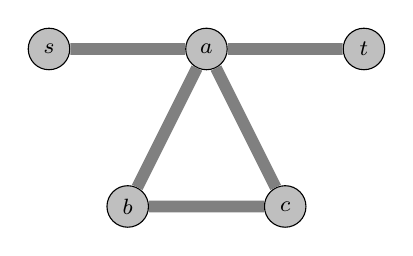
\begin{tikzpicture}
        \tikzstyle{every node}=[circle, fill=lightgray, draw=black, inner sep=2pt, minimum size=1.5em, font=\footnotesize, text=black]
        \tikzstyle{edge}=[gray, line width=1.5mm]
    
        \node (s) at (0,2) {$s$};
        \node (a) at (2,2) {$a$};
        \node (b) at (1,0) {$b$};
        \node (c) at (3,0) {$c$};
        \node (t) at (4,2) {$t$};
    
        \draw[edge] (s) -- (a) -- (b) -- (c) -- (a) -- (t);
    \end{tikzpicture}
    \caption{No odd $s$-$t$-path exist, yet we still have many odd $s$-$t$-walks.}
    \label{figure:small2}
 \end{figure}

Consider \Cref{figure:small2}. There are no odd paths from $s$ to $t$, but we have an infinite amount of odd walks by utilizing the cycles $[a,b,c]$ or $[a,c,b]$ an odd number of times to offset the parity. Our algorithm would perhaps first find an odd walk to $a$, then an even walk to $b$, then an odd walk to $c$, then an even walk to $a$, and lastly an odd walk to $t$. This is one of the two odd $s$-$t$-walks of minimum cost. However, $a$ is visited twice in the walk, once for each parity, and the resulting walk is not a path. Therefore, this algorithm cannot be used to solve \textsc{Shortest Odd Path}.

The main limitation of the algorithm is that the edges in the input graph must have either non-negative weights or no weights at all. Otherwise we cannot guarantee that \pyth{even_dist[u]} and \pyth{odd_dist[u]} have their final, correct values when we scan a vertex $u$. Note that unlike most other algorithms shown in this thesis, this algorithm does not require the input graph to be undirected, it may also be directed.

% \begin{theorem}
%     Let \pyth{(priority, even, u)} be the triple at the front of the queue at any point in the execution of our algorithm.
%     Claim: If \pyth{even} is true and \pyth{even_done[u]} is false, then \pyth{priority} is the cost of the shortest even path from the source to \pyth{u}.

%     \begin{proof}
%     By induction. 

%     The source vertex \pyth{s} has a best possible even cost of \pyth{0}, and initially we have only \pyth{(0, true, s)} in the queue. When that triple is popped the property holds in the base case.

%     \todo[inline]{
%         Burde yoinke beviset herfra: https://web.engr.oregonstate.edu/~glencora/wiki/uploads/dijkstra-proof.pdf

%         Eller herfra: https://community.wvu.edu/~krsubramani/courses/fa05/gaoa/qen/dijk.pdf

%         Eller fra INF234

%         Også si det samme når det er odd, kanskje
%     }

%     \end{proof}
% \end{theorem}

\begin{theorem}
    Let $(G,s,t)$ be an instance of \textsc{Shortest Odd Walk}, let $n := |V|$ and let $m := |E|$.\\
    Claim: the algorithm runs in time at most $O(m \cdot \log m)$, or $O(m \cdot \log n)$ if the graph is simple.
    \begin{proof}
        Because of our \pyth{odd_done} and \pyth{even_done} arrays, we can guarantee that each vertex is scanned at most twice, once for each parity. For each scan, we loop through each of the neighbours in linear time, and consider putting them in the queue. The total cost of the scans is therefore at most $O(m)$. A vertex may be put into the queue many times before it is scanned, in the worst case once for each of its neighbours. That means that we put vertices in the queue at most $O(m)$ times, for a total cost of $O(m)$, and removing all of them takes a total of $O(m \cdot \log m)$. 
        
        The algorithm runs in time at most $O(m) + O(m \cdot \log m) = O(m \cdot \log m)$, which shows the first part of the claim.
        
        If the graph is simple we may simplify the complexity further: $O(m \cdot \log m) \subseteq (m \cdot \log n^2) = O(m \cdot 2 \cdot \log n) = O(m \cdot \log n)$, which shows the second part of the claim.
    \end{proof}
\end{theorem}

To test how well the algorithm scales, we generate 200 Delaunay graphs of sizes 1000, 2000, 3000 and so on until 200 000. We explain how these graphs are generated in \Cref{subsection:delaunay}. For each graph, we have estimated a source and target with the maximum shortest path between them, and run our \textsc{Shortest Odd Walk} algorithm. We take the mediam running time of 10 runs, and plot the results below.

We have also tried to find constants to convert the $O(m \cdot \log m)$ theoretical complexity into a comparable function, and plotted it next to the real practical results.

\begin{center}
    \includesvg[width=0.9\textwidth]{figures/bench_plots/shortest odd walk.svg}    
\end{center}

As we can see, the algorithm easily solves \textsc{Shortest Odd Walk} on graphs of 200000+ vertices in less than 100ms. These results are excellent. Despite having a similiar complexity to the other algorithms in this thesis, this algorithm is still by far the fastest in practice.

Though we discovered it independently, the algorithm is not particularly groundbreaking or in any way creative. Therefore, we do not expect it to be original. It is, however, quite fast, and we are happy with that. The main reason we include it in this thesis is because of its pedagogical value in introducing our main topic: \textsc{Shortest Odd Path}. \todo{Her burde vi finne en eksisterende algoritme og referere til den.}


\chapter{Shortest Odd Path}
\section{Intuition}
Now that we have tried out some algorithms for \textsc{Shortest Odd Walk}, we are finally ready to add the restriction that each vertex is used at most once, and thus solve \textsc{Shortest Odd Path}. The algorithm we are about to present is based on Ulrich Derigs' algorithm \cite{derigs_shortest_odd_path}, though with some improvements.

\subsection{Reduction to \textsc{Shortest Alternating Path}}
\label{reduction}
Consider first another related problem:

\fbox{\parbox{0.94\textwidth}{\textsc{Shortest Alternating Path}\\
    \textbf{Input:} A weighted graph $G := (V, E)$, two vertices $s,t \in V$, and a set $F \subseteq E$\\
    \textbf{Output:} the shortest $s$-$t$-path in $G$ where every other edge used is in $F$.
}}

Derig observed that \textsc{Shortest Odd Path} can be reduced to a special case of \textsc{Shortest Alternating Path}, by constructing what we will refer to as a $\emph{mirror graph}$.

\begin{definition}[Mirror graph]
    Let $G = (V, E)$ be a graph, and $s,t \in V$ be two vertices.
    We construct a new graph $H \sqsupset G$, where for each vertex $u \in V \setminus \{s,t\}$ we add a 'mirror' vertex $u'$, and a connecting 'mirror' edge between them. 
    The vertices in $V(H)$ that are also in $V(G)$ are referred to as the 'real' vertices, and the newly added vertices are referred to as the 'mirror' vertices. In addition, for any vertex $u \in V(H) \setminus \{s,t\}$, real or not, we define $mirror(u)$ as $u$'s mirror on the other side. We usually label mirror vertices with an $'$ at the end of the real counterpart's label.
    For example, if $G$ is the graph in Figure ~\ref{small5}, then Figure ~\ref{small5-2} would be its corresponding mirror graph $H$.
\end{definition}

Our reduction from \textsc{Shortest Odd Path} to \textsc{Shortest Alternating Path} follows:
\begin{enumerate}
    \item Let $(G, s, t)$ be an instance of \textsc{Shortest Odd Path}.
    \item Construct $H$ as the mirror graph of $G$, and let $F$ be the set of mirror edges in $H$. Now $(H, s, t, F)$ is an instance of \textsc{Shortest Alternating Path}.
    \item Let $P'$ be the shortest alternating path of $(H, s, t, F)$, if one exists. If none exist, then we do not have any odd $s$-$t$-paths in $G$ either.
    \item Construct $P$ by filtering out mirror edges from $P'$, and for each edge $(u',v') \in E(H) \setminus (F \cup E(G))$ from the mirror side of $H$ we replace it by the corresponding edge $(u,v) \in E(G)$ from the real side.
    \label{translate_alternating_path}
    \item Now $P$ is the shortest odd $s$-$t$-path in $G$.
\end{enumerate}

\begin{figure}
    \centering
    \includesvg[width=15cm]{figures/graphs/small5.svg}
    \caption{Our input graph $G$, for \textsc{Shortest Odd Path}}
    \label{small5}
\end{figure}

\begin{figure}
    \centering
    \includesvg[width=15cm]{figures/graphs/small5-2.svg}
    \caption{The mirror graph $H$ of $G$, with mirror edges marked in red and mirror vertices labeled with an $'$}
    \label{small5-2}
\end{figure}

For example, if our input $G$ for \textsc{Shortest Odd Path} is Figure ~\ref{small5}, then $H$ and $F$ could look like Figure ~\ref{small5-2}. One of the two possible alternating paths is $P' := [(s,a), (a, a'), (a',b'), (b',b)$, $(b,c), (c,c'), (c',d'), (d',d), (d,t)]$. When we filter out mirror edges and replace edges from the mirror side with their real counterparts, we end up with $P := [(s,a),(a,b),(b,c),(c,d),(d,t)]$, which is one of the two possible odd paths of $G$. 

TODO dette kan kanskje formuleres bedre?

To see why the reduction works, simply observe that for each step we take in the graph, we have to go to the other side of the mirror. If we take another step, we get back to the same side again. It is only when we reach the target vertex $t$ that we do not have to go to the other side. Therefore, to reach a neighbour of $t$, we must have used an even number of mirror edges and an even number of non-mirror edges, and when we take the last step to reach $t$ we have used an odd number of edges and thus found an odd path. If this alternating $s$-$t$-path in $H$ is the shortest such path, then the corresponding path in $G$ must also be the shortest odd $s$-$t$-path in $G$. The reduction works also in the weighted case, as long as each edge $(u',v')$ on the mirror side get the same weight as their real counterpart, and all the mirror edges get the same (usually 0) weight. The interested reader may see \cite{derigs_shortest_odd_path} for more details on this reduction.

Ball and Derigs \cite{shortest_alternating_path} have shown how to efficiently solve \textsc{Shortest Alternating Path}. In their algorithms, subgraphs are shrunk into psuedonodes whenever possible, to make the graph smaller. The drawback is that certain psuedonodes must later be expanded again, which is the most complicated and expensive part of their algorithms. In our case, however, we have a special case of \textsc{Shortest Alternating Path}. The set $F$ is, with the exception of $s$ and $t$, a perfect matching of $H$, and we will therefore never have to expand psuedonodes after shrinking them. The curious reader may visit \cite{shortest_alternating_path} for more on these algorithms and why our almost-perfect matching is a simpler case.

\subsection{The idea for our \textsc{Shortest Alternating Path} algorithm}
We will explain the general idea of our algorithm by following an example, and solve for the graph in figure \ref{small5}. First we construct the mirror graph like explained in \ref{reduction}, to produce the graph in figure \ref{small5-2}. Then we initialize an empty priority queue of vertices and edges to be scanned. For each vertex $u \in V(H)$, we denote
\begin{itemize}
    \item $d^+_u :=$ the length of the shortest alternating $s$-$u$-path ending on a mirror edge
    \item $d^-_u :=$ the length of the shortest alternating $s$-$u$-path ending on a non-mirror edge
    \item $pred_u :=$ the last edge used to find $u$'s most recent value for $d^-_u$
\end{itemize}

Initally these are either $\infty$ or undefined, except for the source vertex $s$, where we can set $d^+_s := 0$. Then, for each edge $(s,u) \in N(s)$, we can set $d^-_u := weight((s,u))$, $pred_u := (s,u)$, and add $u$ to our priority queue with priority $2 \cdot weight((s,u))$.

We visualize it like in the diagram below. Each vertex $u$ has its values for $d^-_u$ and $d^+_u$ to its top left and top right, respectively.

\includesvg[width=12cm]{figures/example_story/example-story1.svg}

The first and only vertex in the queue is $A$. We pop it, set $d^+_{A'} := d^-_A$, and 'scan' $A'$. By that, we mean to look at each neighbour $e \in N(A')$, and see if our new value $d^+_{A'} + weight(e)$ is better than the previous value $d^-_{to(edge)}$. That is the case for both $B'$ and $C'$, so we update their values and add them to the queue. Their priorities in the queue is equal to twice their $d^-$ values, which is $2 \cdot 2 = 4$ for both of them.

\includesvg[width=12cm]{figures/example_story/example-story2.svg}

The next vertex in the queue is $B'$, so we set $d^+_B := d^-_{B'}$ and scan $B'$:

\includesvg[width=12cm]{figures/example_story/example-story3.svg}

Now $C'$ is the next in the queue, we set $d^+_C := d^-{C'}$ and scan $C'$. This is where the interesting part happens: now we have set both $d^+$ and $d^-$ for $B$ and $C$, and that means that we have found an odd cycle in the graph. The edge between them, $(B,C)$, is called the \emph{blossom edge}, and is marked in green. We add $(B,C)$ to the queue, with the priority $d^+_C + d^+_B + weight((B,C))$.

\includesvg[width=12cm]{figures/example_story/example-story4.svg}

Next up is to scan this blossom edge, and compute its corresponding odd cycle by backtracking from $C$ and $B$ until they meet at $A'$. To visualize the cycle, we like to 'stretch out' the graph a little, and draw it like below. Note that some of the edges are omitted for clarity. Now we can see that the cycle consists of [$A',C',C,B,B',A'$]. We call the set $\mathbb{B} := \{C',C,B,B'\}$ a \emph{blossom}, and $A'$ the \emph{base} of the blossom, inspired by the famous Blossom algorithm by \cite{blossom}.

\includesvg[width=12cm]{figures/example_story/example-story5.svg}

The first reason why we care about this blossom is because now we can immedeately set the final, optimal $d^-$ and $d^+$ for all the vertices in the blossom. That is because we now have two alternating paths to each vertex, one goes around the cycle while the other takes the shortcut. One of these ends up on a mirror edge, and the other on a normal edge, and both are optimal. For example, to go from $S$ to $C'$, we can either go through [$S,A,A',C'$] with a cost of $d^-_C$, or go along [$S,A,A',B',B,C,C'$] with a cost of $d^+_C$.

More specifically, for each $u \in \mathbb{B}$: \begin{itemize}
    \item If $d^+_u = \infty$, we set $d^+_u = d^-_{mirror(u)}$.
    \item If we can improve $d^-_u$ by coming from its neighbour in the blossom, we do so.
\end{itemize}
After all these values have been set, we immedeately scan all the vertices in $\mathbb{B}$ that just received values for $d^+$. In this example we scan $C'$ and $B'$, and discover $D'$. Unfortunately, since this is a very small blossom we don't have any vertices that receive new values for $d^-$.

\includesvg[width=12cm]{figures/example_story/example-story6.svg}

% TODO føler dette kan skrives bedre
The second reason we compute the blossom is that we no longer care much about the individual vertices in $\mathbb{B}$, and can shrink it into just the base $A'$. We will still scan vertices like $C$ from the queue as before, but whenever we are backtracking to compute blossoms we can skip the verties in $\mathbb{B}$ entirely and go straight to the base $A'$ instead. In this example, in a few iterations the algorithm will find either $(D',A')$ or $(D,A')$ as a blossom edge, with just $\{D,D'\}$ as its blossom and $A'$ as the base here as well. If we didn't contract the previous blossom, this new blossom would instead consist of $\{C',C,B,B',D,D'\}$, but we are already completely done with most of those vertices and computing all of it again would be a waste. Therefore we shrink them. 

If the reader is familiar with the more general \textsc{Shortest Alternating Path} algorithm \cite{shortest_alternating_path} or the original blossom algorithm \cite{blossom}, and worry that such psuedonodes often have to be expanded again, then remember that in our case the set $F$ is an almost-perfect matching and those cases never happen. % TODO trenger vi si dette? Droppe det? Formulere det annerledes?

\includesvg[width=12cm]{figures/example_story/example-story7.svg}

Let us now skip a few steps, until $T$ eventually reaches the front of the queue. At that point we have that $d^-_T = 5$, and that is also the cost of the shortest odd path in our original input graph. To compute the exact path we can backtrack from $T$ to $S$ and then translate that path as described in step \ref{translate_alternating_path} of our reduction in \ref{reduction}. We end up with the path [$(S,A),(A,B),(B,C),(C,D),(D,T)$], which is the shortest odd $S$-$T$-path in the graph.

\section{Psuedocode}

\begin{lstlisting}[caption={Main},label=Listing,mathescape=true]
fn main(Graph input_graph, int s, int t) -> Option<(int, List<Edge>)> {
    init(input_graph, s, t);

    while ! control() {}

    if d_minus[t] == $\infty$ {
        // The graph is a no-instance, no odd s-t-paths exist
        return None;
    }

    Edge current_edge = pred[t];
    List<Edge> path = [current_edge];
    while from(current_edge) != s {
        current_edge = pred[mirror(from(current_edge))];
        if from(current_edge) < input_graph.n() {
            path.push(current_edge);
        }
        else {
            path.push(shift_edge_by(current_edge, -input_graph.n()));
        }
    }
    return Some(d_minus[t], path);
}
\end{lstlisting}

\begin{lstlisting}[caption={Initialization},label=Listing,mathescape=true]
fn init(Graph input_graph, int s, int t) {
    graph = create_mirror_graph(input_graph);

    for u in 0..n {
        d_plus[u] = $\infty$;
        d_minus[u] = $\infty$;
        pred[u] = null;
        completed[u] = false;
    }
    d_plus[s] = 0;
    completed[s] = true;

    for edge in graph[s] {
        pq.push(Vertex(weight(edge), to(edge)));
        d_minus[to(edge)] = weight(edge);
        pred[to(edge)] = e;
    }
}
\end{lstlisting}

\begin{lstlisting}[caption={Control, the main loop},label=Listing,mathescape=true]
fn control() -> bool {
    while ! pq.is_empty() {
        match pq.top() {
            Vertex(_, u) => {
                if completed[u] {
                    pq.pop();
                }
                else {
                    break;
                }
            },
            Blossom(_, edge) => {
                if base_of(from(edge)) == base_of(to(edge)) {
                    pq.pop();
                }
                else {
                    break;
                }
            }
        }
    }

    if pq.is_empty() {
        // No odd s-t-paths in G exist :(
        return true;
    }
    match pq.pop() {
        Vertex(delta, l) => {
            if l == t {
                // We have found a shortest odd s-t-path has been found :)
                return true;
            }
            grow(l, delta)
        }
        Blossom(delta, edge) => {
            blossom(e);
        }
    }
    return false;
}
\end{lstlisting}

\begin{lstlisting}[caption={Grow},label=Listing,mathescape=true]
fn grow(int l, int delta) {
    int k = mirror(l);
    d_plus[k] = delta;
    scan(k);
}
\end{lstlisting}

\begin{lstlisting}[caption={Scan},label=Listing,mathescape=true]
fn scan(int u) {
    completed[u] = true;
    int dist_u = d_plus[u];
    for edge in graph[u] {
        int v = to(edge);
        int new_dist_v = dist_u + weight(edge);

        if ! completed[v] {
            if new_dist_v < d_minus[v] {
                d_minus[v] = new_dist_v;
                pred[v] = edge;
                pq.push(Vertex(new_dist_v, v));
            }
        }
        else if d_plus[v] < $\infty$ and base_of(u) != base_of(v) {
            pq.push(Blossom(d_plus[u] + d_plus[v] + weight(edge)));
            if new_dist_v < d_minus[v] {
                d_minus[v] = new_dist_v;
                pred[v] = e;
            }
        }
    }
}

\end{lstlisting}

\begin{lstlisting}[caption={Blossom},label=Listing,mathescape=true]
fn blossom(Edge edge) {
    (int, List<Edge>, List<Edge>) (b, p1, p2) = backtrack_blossom(edge);

    List<int> to_scan1 = set_blossom_values(p1);
    List<int> to_scan2 = set_blossom_values(p2);

    set_edge_bases(b, p1);
    set_edge_bases(b, p2);

    for u in to_scan1 {
        scan(u);
    }
    for v in to_scan2 {
        scan(v);
    }
}
\end{lstlisting}

\begin{lstlisting}[caption={Backtrack blossom},label=Listing,mathescape=true]
fn backtrack_blossom(Edge edge) -> (int, List<Edge>, List<Edge>){
    // TODO
}
\end{lstlisting}


\begin{lstlisting}[caption={Set blossom values},label=Listing,mathescape=true]
fn set_blossom_values(List<Edge> path) -> List<int> {
    List<int> to_scan = [];

    for edge in path {
        int u = from(edge);
        int v = to(edge);
        int w = weight(edge);
        in_current_cycle[u] = false;
        in_current_cycle[v] = false;

        // We can set a d_minus
        if d_plus[v] + w < d_minus[u] {
            d_minus[u] = d_plus[v] + w;
            pred[u] = reverse(edge);
        }

        int m = mirror(u);
        // We can set a d_plus, and scan it
        if d_minus[u] < d_plus[m] {
            d_plus[m] = d_minus[u];
            to_scan.push(m);
        }
    }

    return to_scan;
}
\end{lstlisting}

\begin{lstlisting}[caption={Set edge bases},label=Listing,mathescape=true]
fn set_edge_bases(int b, List<Edge> path) {
    for edge in path {
        let u = from(edge);
        let m = mirror(edge);
        set_base(u, b);
        set_base(m, b);
    }
}
\end{lstlisting}


\begin{lstlisting}[caption={Basis},label=Listing,mathescape=true]
fn init(Graph input_graph, int s, int t) {
    // omitted
    Graph graph = create_mirror_graph(input_graph, s, t);
    for u in 0..graph.n() {
        basis[u] = u;
    }
    // omitted
}
fn set_base(int b, int u) {
    basis[u] = b;
}
fn get_base(int u) -> int {
    if u != basis[u] {
        basis[u] = get_base(basis[u]);
    }
    return basis[u];
}

\end{lstlisting}

\section{Notes on implementing the psuedocode}
\section{Analysis}

\subsection{Complexity}

\subsection{Benchmarking methodology}

\subsection{Results}

\subsection{Discussion}

\chapter{Network Diversion}
\section{Intuition}
\subsection{Detour paths}
\label{section:subdividing-detours}
Before we reveal the algorithm for Network Diversion, we will first look at a curious little problem that we call \textsc{Shortest Detour Path}. Instead of deleting edges to force all paths to go through a certain edge, we want to purposefully pass through that edge and look for the shortest path that does. Perhaps we are going on a road trip, and we want to stop at a specific gas station along a road to say hi to our friend Mike who works there. And because this is a road trip, we do not want to drive along the same roads multiple times, that would be boring.

\problem
{Shortest Detour Path}
{a graph $G$, two vertices $s,t \in V$, and a 'detour' edge $d \in E$}
{an $s$-$t$-path in $G$ of minimum cost, that goes through the detour $d$}

There is no obvious way to solve \textsc{Shortest Detour Path}. One might attempt to concatenate the shortest $s$-$\from(d)$-path and the shortest $\too(d)$-$t$-path, but those two paths might overlap and reuse the same vertices, and therefore would their concatenation not necessarily be a path but instead merely a walk.

Instead, we create a new graph $H$, by subdividing all edges in $G$ \emph{except} $d$, as seen in \Cref{figure:subdividing-detours}. The key point to see here is that any odd $s$-$t$-path in $H$ must necessarily go through the detour, otherwise it would not be odd. We can visualize it by 'stepping through' the edges in $H$. If we start on our right leg, then in the beginning every time we reach a vertex that is also in $G$, we reach it by stepping on our left leg. That continues until we use the detour edge, and from then on we step on all vertices from $G$ using our right leg. If we require that we end at $t$ on our right leg, then the path must be odd, and any odd path must go through the detour. Therefore we can simply run our \textsc{Shortest Odd Path} algorithm on $H$, and if such a path exists we can reverse the subdivision of the edges in the path and the result is the \textsc{Shortest Detour Path} in $G$.

\begin{figure}[H]
    \centering
    \begin{subfigure}{.45\textwidth}
        \centering
        \scalebox{0.88}{
            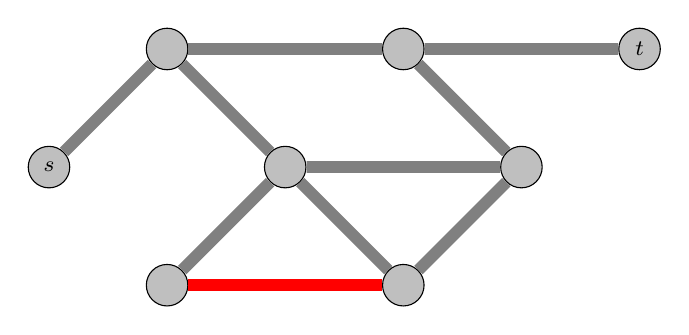
\begin{tikzpicture}
                \tikzstyle{every node}=[circle, fill=lightgray, draw=black, inner sep=2pt, minimum size=1.5em, font=\footnotesize, text=black]
                \tikzstyle{edge}=[gray, line width=1.5mm]
            
                \node (s) at (0,0) {$s$};
                \node (a) at (1.5,1.5) {};
                \node (b) at (3,0) {};
                \node (c) at (1.5,-1.5) {};
                \node (d) at (4.5,-1.5) {};
                \node (e) at (6,0) {};
                \node (f) at (4.5,1.5) {};
                \node (t) at (7.5,1.5) {$t$};
            
                \draw[edge] (s) -- (a) -- (b) -- (e);
                \draw[edge] (c) -- (b) -- (d) -- (e) -- (f) -- (t);
                \draw[edge] (a) -- (f);
            
                \tikzstyle{edge}=[red, line width=1.5mm]
                \draw[edge] (c) -- (d);
            \end{tikzpicture}
        }
        \caption{An instance of \textsc{Shortest Deour Path}, the detour marked in red.}
        \label{figure:detour}
    \end{subfigure}\hfill%
    \begin{subfigure}{.45\textwidth}
        \centering
        \scalebox{0.88}{
            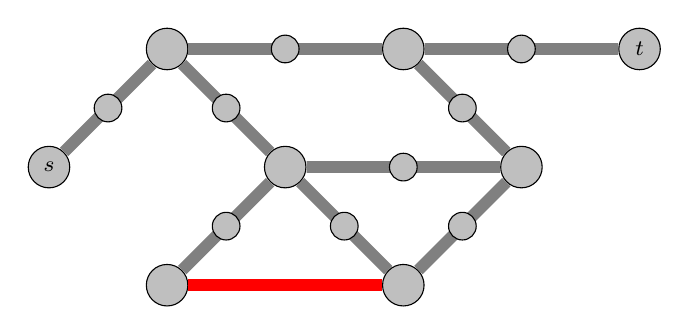
\begin{tikzpicture}
                \tikzstyle{every node}=[circle, fill=lightgray, draw=black, inner sep=2pt, minimum size=1.5em, font=\footnotesize, text=black]
                \tikzstyle{edge}=[gray, line width=1.5mm]
            
                \node (s) at (0,0) {$s$};
                \node (a) at (1.5,1.5) {};
                \node (b) at (3,0) {};
                \node (c) at (1.5,-1.5) {};
                \node (d) at (4.5,-1.5) {};
                \node (e) at (6,0) {};
                \node (f) at (4.5,1.5) {};
                \node (t) at (7.5,1.5) {$t$};
            
                \draw[edge] (s) -- (a) -- (b) -- (e);
                \draw[edge] (c) -- (b) -- (d) -- (e) -- (f) -- (t);
                \draw[edge] (a) -- (f);
            
                \tikzstyle{edge}=[red, line width=1.5mm]
                \draw[edge] (c) -- (d);

                \tikzstyle{every node}=[circle, fill=lightgray, draw=black, inner sep=2pt, minimum size=1em, font=\footnotesize, text=black]
                \node (sa) at (0.75,0.75) {};
                \node (af) at (3,1.5) {};
                \node (ab) at (2.25,0.75) {};
                \node (bc) at (2.25,-0.75) {};
                \node (bd) at (3.75,-0.75) {};
                \node (be) at (4.5,0) {};
                \node (de) at (5.25,-0.75) {};
                \node (ef) at (5.25,0.75) {};
                \node (ft) at (6,1.5) {};
            \end{tikzpicture}
        }
        \caption{All edges except the detour have been subdivided, to create an instance of \textsc{Shortest Odd Path}.}
        \label{figure:subdivided-detour}
    \end{subfigure}%
    \caption{\textsc{Shortest Detour Path} reduced to \textsc{Shortest Odd Path} by subdividing all edges except the detour.}
    \label{figure:subdividing-detours}
\end{figure}

If we extend the problem to have multiple detour edges, where we have to go through all of them in any order, then our idea will not work\footnote{This is a good thing, because otherwise we would have solved the \textsc{Traveling Salesman Problem} in polynomial time and complexity theory as we know it would break down.}.
The problem is that we have no way of knowing whether we have used the marked edges 1, 3, or 5, etc. times, because in all of them we hit vertices from $G$ using our right leg. We can, however, use this idea to find paths that use a certain set of edges an odd amount of times. As it turns out, that is exactly what we need to solve \textsc{Network Diversion}.

\subsection{From a dual path to a real diversion}
Remember, we want to find a minimum minimal $s$-$t$-cut in $G$ that includes the diversion edge $d$.

Instead of looking for a minimal cut in $G$, let us look for a simple cycle in the dual graph $G^\star$, as is explained to be equivalent in \Cref{fact:dual-cycle-is-real-cut}. We can do this by finding a path in $G^\star$ from and to the left and right faces of $d$, without using $d^\star$ itself, and then adding $d^\star$ at the end to complete the cycle. If the path found is also the shortest such path, then it corresponds to the \emph{minimum} minimal cut in $G$ that uses $d$, though it is not necessarily an $s$-$t$-cut.

To force $s$ and $t$ to end up in different components after the cut, we need some additional details. First, we find any $s$-$t$-path in $G$, not necessarily the shortest path. Then we subdivide all the edges in the dual graph \emph{except} those who cross edges on the found $s$-$t$-path. Now we can look for the shortest \emph{odd} path from and two the left and right faces of $d$ in the subdivided dual graph, and add $d^\star$ at the end to make it a cycle. Like before, this corresponds to a minimum minimal cut in $G$ that uses $d$, but now it must also cross the edges in the found $s$-$t$-path an odd number of times, as explained in \Cref{section:subdividing-detours}. 

This cycle, and the found $s$-$t$-path, can be interpreted as curves in our embedding. The cycle can additionally be interpreted as a Jordan curve, and by the Jordan Curve Theorem, the cycle divides the plane into an 'inside' and an 'outside'. Since the curve of the $s$-$t$-path crosses the curve of the cycle an odd number of times, exactly one of its endpoints must be on the inside, as illustrated in \Cref{figure:jordan-curve-cuts}. The endpoints are $s$ and $t$, meaning that $s$ and $t$ end up in different components after the cut. It follows that this cut is an $s$-$t$-cut in $G$, specifically a minimum minimal $s$-$t$-cut in $G$ that uses $d$.

This is the main idea for our algorithm. Note that we did not come up with this idea ourselves, but have to thank Pål Grønås Drange \cite{source:pål} for his as for now unpublished work on the subject.

\begin{figure}[H]
    \centering
    \begin{subfigure}{.30\textwidth}
        \centering
        \includesvg[width = 0.8\textwidth]{figures/jordan_curves/one_crossing.svg}
        \caption{The path crosses the cycle once, so exactly one of the endpoints is on the inside.}
    \end{subfigure}\hfill%
    \begin{subfigure}{.30\textwidth}
        \centering
        \includesvg[width = 0.8\textwidth]{figures/jordan_curves/two_crossings.svg}
        \caption{The path crosses the cycle twice, both endpoints are on the outside.}
    \end{subfigure}\hfill%
    \begin{subfigure}{.30\textwidth}
        \centering
        \includesvg[width = 0.8\textwidth]{figures/jordan_curves/three_crossings.svg}
        \caption{The path crosses the cycle thrice, so the endpoints must end up on either side of the cycle.}
    \end{subfigure}
    \caption{The two endpoints of a path end up on different sides of a cycle if and only if it crosses the cycle an odd number of times.}
    \label{figure:jordan-curve-cuts}
\end{figure}

\subsection{The algorithm}
\label{subsection:network-diversion-example}
We will explain the algorithm by following an example. We want to find the minimum minimal $s$-$t$-cut that includes the diversion edge marked in red. 

\begin{center}
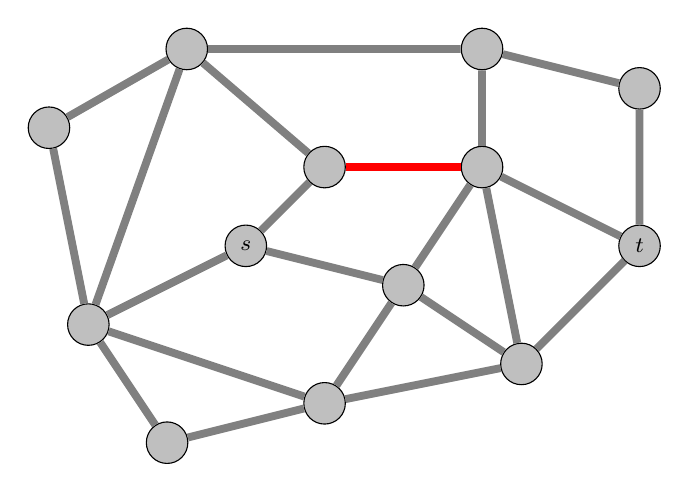
\begin{tikzpicture}
    \tikzstyle{every node}=[circle, fill=lightgray, draw=black, inner sep=2pt, minimum size=1.5em, font=\footnotesize, text=black]
    \tikzstyle{edge}=[gray, line width=1mm]

    \node (s) at (0,0) {$s$};
    \node (a) at (2,-0.5) {};
    \node (b) at (1,-2) {};
    \node (c) at (1,1) {};
    \node (d) at (3.5,-1.5) {};
    \node (e) at (3,1) {};
    \node (f) at (-2,-1) {};
    \node (t) at (5,0) {$t$};
    \node (g) at (-1,-2.5) {};
    \node (h) at (3,2.5) {};
    \node (i) at (-0.75,2.5) {};
    \node (j) at (5,2) {};
    \node (k) at (-2.5,1.5) {};

    \draw[edge] (t) -- (j) -- (h) -- (i) -- (k) -- (f) -- (g) -- (b) -- (d) -- (e) -- (h);
    \draw[edge] (s) -- (c) -- (i) -- (f) -- (s);
    \draw[edge] (f) -- (b) -- (a) -- (d) -- (t);
    \draw[edge] (s) -- (a) -- (e) -> (t);

    \tikzstyle{edge}=[red, line width=1mm]
    \draw[edge] (c) -- (e);
\end{tikzpicture}
\end{center}

First, we find any $s$-$t$-path that does not use the diversion edge. It does not necessarily have to be the shortest path. We have marked such a path in green below.

\begin{center}
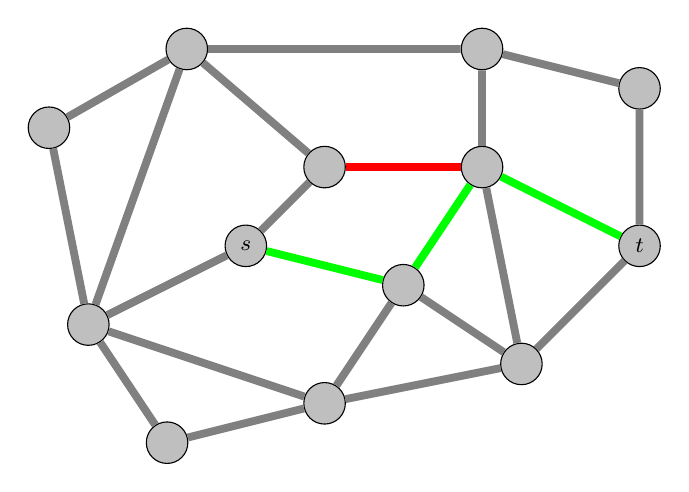
\begin{tikzpicture}
    \tikzstyle{every node}=[circle, fill=lightgray, draw=black, inner sep=2pt, minimum size=1.5em, font=\footnotesize, text=black]
    \tikzstyle{edge}=[gray, line width=1mm]

    \node (s) at (0,0) {$s$};
    \node (a) at (2,-0.5) {};
    \node (b) at (1,-2) {};
    \node (c) at (1,1) {};
    \node (d) at (3.5,-1.5) {};
    \node (e) at (3,1) {};
    \node (f) at (-2,-1) {};
    \node (t) at (5,0) {$t$};
    \node (g) at (-1,-2.5) {};
    \node (h) at (3,2.5) {};
    \node (i) at (-0.75,2.5) {};
    \node (j) at (5,2) {};
    \node (k) at (-2.5,1.5) {};

    \draw[edge] (t) -- (j) -- (h) -- (i) -- (k) -- (f) -- (g) -- (b) -- (d) -- (e) -- (h);
    \draw[edge] (s) -- (c) -- (i) -- (f) -- (s);
    \draw[edge] (f) -- (b) -- (a) -- (d) -- (t);

    \tikzstyle{edge}=[red, line width=1mm]
    \draw[edge] (c) -- (e);

    \tikzstyle{edge}=[green, line width=1mm]
    \draw[edge] (s) -- (a) -- (e) -> (t);
\end{tikzpicture}
\end{center}

Next up is to compute the dual graph. We delete the dual edge that crosses the diversion edge and color the rest in blue here. Note that we have omitted the outside face and its edges in this visualization, otherwise we would have a much too cluttered illustration.

\begin{center}
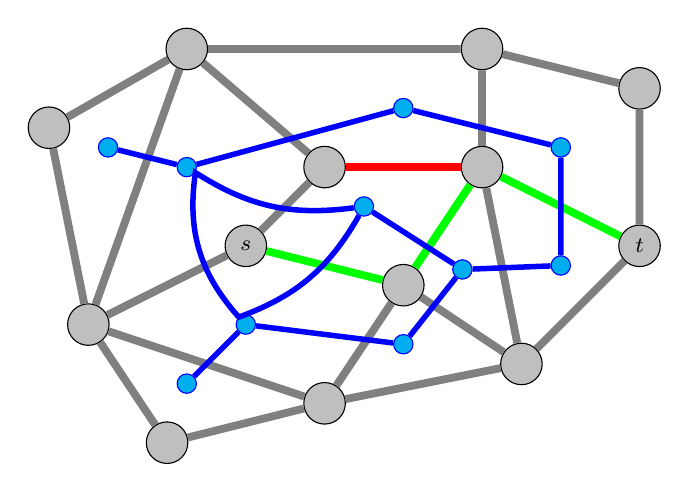
\begin{tikzpicture}
    \tikzstyle{every node}=[circle, fill=lightgray, draw=black, inner sep=2pt, minimum size=1.5em, font=\footnotesize, text=black]
    \tikzstyle{edge}=[gray, line width=1mm]

    \node (s) at (0,0) {$s$};
    \node (a) at (2,-0.5) {};
    \node (b) at (1,-2) {};
    \node (c) at (1,1) {};
    \node (d) at (3.5,-1.5) {};
    \node (e) at (3,1) {};
    \node (f) at (-2,-1) {};
    \node (t) at (5,0) {$t$};
    \node (g) at (-1,-2.5) {};
    \node (h) at (3,2.5) {};
    \node (i) at (-0.75,2.5) {};
    \node (j) at (5,2) {};
    \node (k) at (-2.5,1.5) {};

    \draw[edge] (t) -- (j) -- (h) -- (i) -- (k) -- (f) -- (g) -- (b) -- (d) -- (e) -- (h);
    \draw[edge] (s) -- (c) -- (i) -- (f) -- (s);
    \draw[edge] (f) -- (b) -- (a) -- (d) -- (t);

    \tikzstyle{edge}=[red, line width=1mm]
    \draw[edge] (c) -- (e);

    \tikzstyle{edge}=[green, line width=1mm]
    \draw[edge] (s) -- (a) -- (e) -> (t);

    \tikzstyle{every node}=[circle, draw=blue, fill=cyan, inner sep=2pt, minimum size=0.7em]
    \node (aces) at (1.5,0.5) {};
    \node (cehi) at (2,1.75) {};
    \node (ehjt) at (4,1.25) {};
    \node (det) at (4,-0.25) {};
    \node (ade) at (2.75,-0.3) {};
    \node (abd) at (2,-1.25) {};
    \node (abfs) at (0,-1) {};
    \node (bfg) at (-0.75,-1.75) {};
    \node (cifs) at (-0.75,1) {};
    \node (fik) at (-1.75,1.25) {};

    \tikzstyle{edge}=[blue, line width=0.7mm]
    \draw[edge] (fik) -- (cifs) -- (cehi) -- (ehjt) -- (det) -- (ade) -- (abd) -- (abfs) -- (bfg);
    \draw[edge] (ade) -- (aces) to [bend left=20] (cifs) to [bend right=25] (abfs) to [bend right=20] (aces); 
\end{tikzpicture}
\end{center}

Now we subdivide all the edges in the dual graph except those that cross the path in green.

\begin{center}
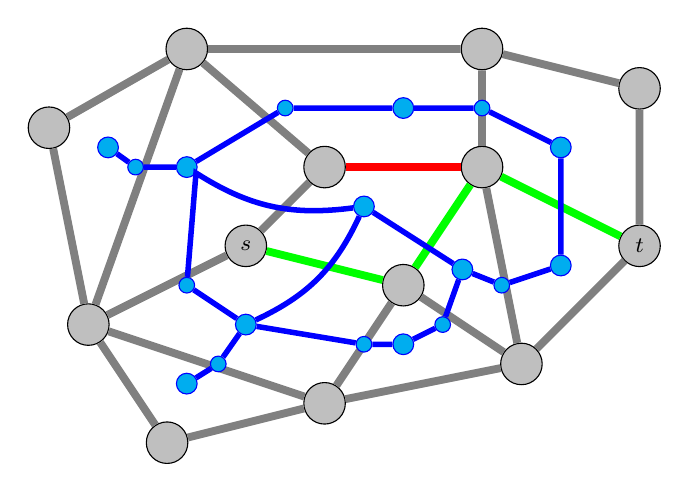
\begin{tikzpicture}
    \tikzstyle{every node}=[circle, fill=lightgray, draw=black, inner sep=2pt, minimum size=1.5em, font=\footnotesize, text=black]
    \tikzstyle{edge}=[gray, line width=1mm]

    \node (s) at (0,0) {$s$};
    \node (a) at (2,-0.5) {};
    \node (b) at (1,-2) {};
    \node (c) at (1,1) {};
    \node (d) at (3.5,-1.5) {};
    \node (e) at (3,1) {};
    \node (f) at (-2,-1) {};
    \node (t) at (5,0) {$t$};
    \node (g) at (-1,-2.5) {};
    \node (h) at (3,2.5) {};
    \node (i) at (-0.75,2.5) {};
    \node (j) at (5,2) {};
    \node (k) at (-2.5,1.5) {};

    \draw[edge] (t) -- (j) -- (h) -- (i) -- (k) -- (f) -- (g) -- (b) -- (d) -- (e) -- (h);
    \draw[edge] (s) -- (c) -- (i) -- (f) -- (s);
    \draw[edge] (f) -- (b) -- (a) -- (d) -- (t);

    \tikzstyle{edge}=[red, line width=1mm]
    \draw[edge] (c) -- (e);

    \tikzstyle{edge}=[green, line width=1mm]
    \draw[edge] (s) -- (a) -- (e) -> (t);

    \tikzstyle{every node}=[circle, draw=blue, fill=cyan, inner sep=2pt, minimum size=0.75em]
    \node (aces) at (1.5,0.5) {};
    \node (cehi) at (2,1.75) {};
    \node (ehjt) at (4,1.25) {};
    \node (det) at (4,-0.25) {};
    \node (ade) at (2.75,-0.3) {};
    \node (abd) at (2,-1.25) {};
    \node (abfs) at (0,-1) {};
    \node (bfg) at (-0.75,-1.75) {};
    \node (cifs) at (-0.75,1) {};
    \node (fik) at (-1.75,1.25) {};


    \tikzstyle{every node}=[circle, draw=blue, fill=cyan, inner sep=2pt, minimum size=0.35em]
    \node (fi) at (-1.4,1) {};
    \node (fs) at (-0.75,-0.5) {};
    \node (bf) at (-0.35,-1.5) {};
    \node (ci) at (0.5,1.75) {};
    \node (eh) at (3,1.75) {};
    \node (de) at (3.25,-0.5) {};
    \node (ad) at (2.5,-1) {};
    \node (ab) at (1.5,-1.25) {};

    \tikzstyle{edge}=[blue, line width=0.7mm]
    \draw[edge] (fik) -- (fi) -- (cifs) -- (ci) -- (cehi) -- (eh) -- (ehjt) -- (det) -- (de) -- (ade) -- (ad) -- (abd) -- (ab) -- (abfs) -- (bf) -- (bfg);
    \draw[edge] (ade) -- (aces) to [bend left=20] (cifs) -- (fs) -- (abfs) to [bend right=20] (aces);    
\end{tikzpicture}
\end{center}

The last step is to find the shortest odd path in the subdivided dual graph from and to the regions to the left and right of the diversion edge, using our newfound favorite algorithm. If we find such a path, we know that it must cross the $s$-$t$-path in green an odd number of times. If we add the dual equivalent of the diversion edge to the path to create a cycle, then we know that this cycle goes around either $s$ or $t$, but not both. We illustrate the cycle below, this time in orange in an attempt to not run out of colors.

\begin{center}
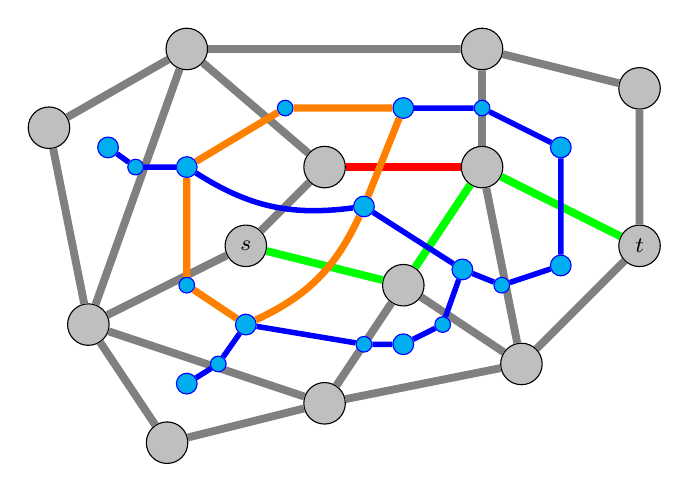
\begin{tikzpicture}
    \tikzstyle{every node}=[circle, fill=lightgray, draw=black, inner sep=2pt, minimum size=1.5em, font=\footnotesize, text=black]
    \tikzstyle{edge}=[gray, line width=1mm]

    \node (s) at (0,0) {$s$};
    \node (a) at (2,-0.5) {};
    \node (b) at (1,-2) {};
    \node (c) at (1,1) {};
    \node (d) at (3.5,-1.5) {};
    \node (e) at (3,1) {};
    \node (f) at (-2,-1) {};
    \node (t) at (5,0) {$t$};
    \node (g) at (-1,-2.5) {};
    \node (h) at (3,2.5) {};
    \node (i) at (-0.75,2.5) {};
    \node (j) at (5,2) {};
    \node (k) at (-2.5,1.5) {};

    \draw[edge] (t) -- (j) -- (h) -- (i) -- (k) -- (f) -- (g) -- (b) -- (d) -- (e) -- (h);
    \draw[edge] (s) -- (c) -- (i) -- (f) -- (s);
    \draw[edge] (f) -- (b) -- (a) -- (d) -- (t);

    \tikzstyle{edge}=[red, line width=1mm]
    \draw[edge] (c) -- (e);

    \tikzstyle{edge}=[green, line width=1mm]
    \draw[edge] (s) -- (a) -- (e) -> (t);

    \tikzstyle{every node}=[circle, draw=blue, fill=cyan, inner sep=2pt, minimum size=0.75em]
    \node (aces) at (1.5,0.5) {};
    \node (cehi) at (2,1.75) {};
    \node (ehjt) at (4,1.25) {};
    \node (det) at (4,-0.25) {};
    \node (ade) at (2.75,-0.3) {};
    \node (abd) at (2,-1.25) {};
    \node (abfs) at (0,-1) {};
    \node (bfg) at (-0.75,-1.75) {};
    \node (cifs) at (-0.75,1) {};
    \node (fik) at (-1.75,1.25) {};


    \tikzstyle{every node}=[circle, draw=blue, fill=cyan, inner sep=2pt, minimum size=0.35em]
    \node (fi) at (-1.4,1) {};
    \node (fs) at (-0.75,-0.5) {};
    \node (bf) at (-0.35,-1.5) {};
    \node (ci) at (0.5,1.75) {};
    \node (eh) at (3,1.75) {};
    \node (de) at (3.25,-0.5) {};
    \node (ad) at (2.5,-1) {};
    \node (ab) at (1.5,-1.25) {};

    \tikzstyle{edge}=[blue, line width=0.7mm]
    \draw[edge] (fik) -- (fi) -- (cifs);
    \draw[edge] (cehi) -- (eh) -- (ehjt) -- (det) -- (de) -- (ade) -- (ad) -- (abd) -- (ab) -- (abfs) -- (bf) -- (bfg);
    \draw[edge] (ade) -- (aces) to [bend left=20] (cifs);

    \tikzstyle{edge}=[orange, line width=0.9mm]
    \draw[edge] (cehi) -- (ci) -- (cifs) -- (fs) -- (abfs) to [bend right=20] (aces);
    \draw[edge] (aces) -- (cehi);
\end{tikzpicture}
\end{center}

With this, we finally have our diversion set. Simply delete the edges in the original graph that cross the cycle we found and colored in orange, except for the diversion edge of course. We end up with a graph where all $s$-$t$-paths must pass through the diversion edge. The problem is solved.

\begin{center}
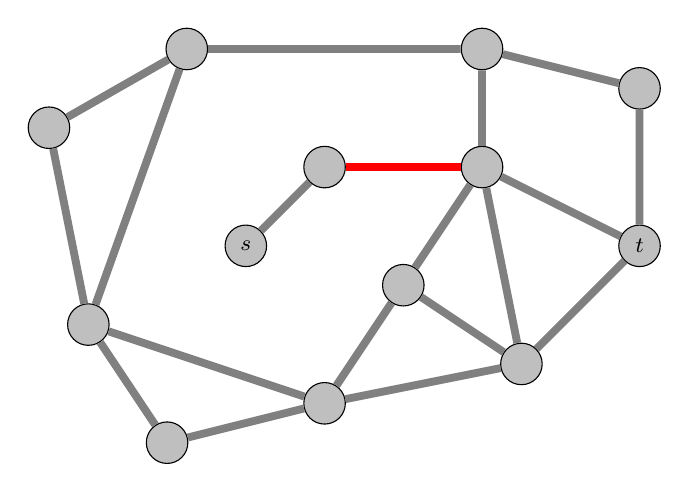
\begin{tikzpicture}
    \tikzstyle{every node}=[circle, fill=lightgray, draw=black, inner sep=2pt, minimum size=1.5em, font=\footnotesize, text=black]
    \tikzstyle{edge}=[gray, line width=1mm]

    \node (s) at (0,0) {$s$};
    \node (a) at (2,-0.5) {};
    \node (b) at (1,-2) {};
    \node (c) at (1,1) {};
    \node (d) at (3.5,-1.5) {};
    \node (e) at (3,1) {};
    \node (f) at (-2,-1) {};
    \node (t) at (5,0) {$t$};
    \node (g) at (-1,-2.5) {};
    \node (h) at (3,2.5) {};
    \node (i) at (-0.75,2.5) {};
    \node (j) at (5,2) {};
    \node (k) at (-2.5,1.5) {};

    \draw[edge] (t) -- (j) -- (h) -- (i) -- (k) -- (f) -- (g) -- (b) -- (d) -- (e) -- (h);
    \draw[edge] (c) -- (s);
    \draw[edge] (a) -- (e) -- (t);
    \draw[edge] (i) -- (f) -- (b) -- (a) -- (d) -- (t);

    \tikzstyle{edge}=[red, line width=1mm]
    \draw[edge] (c) -- (e);
\end{tikzpicture}
\end{center}
\section{Psuedocode}
\begin{lstlisting}[caption={Main},label=Listing,mathescape=true]
network_diversion(PlanarGraph graph, s, t, Edge diversion) -> Option<(int, List<Edge>)> {
    let `path` be any s-t-path that does not use the diversion edge;
}
\end{lstlisting}
\section{Analysis}

\subsection{Limitations}
Whether \textsc{Network Diversion} in the general case can be solved in polynomial time is still an open problem.
This algorithm does not solve the general case, but rather the special case where the input graph...
\begin{itemize}
    \item is planar,
    \item is undirected,
    \item has edges of either non-negative weights or no weights at all.
\end{itemize}

In addition, even though the algorithm as described here will also work on non-simple graphs, we implemented the algorithm with the assumption that the graph is simple. See \Cref{chapter:codebase} for more details. \todo{vurder å skrive dette i kodekapitlet istedet. Eller også ta med at vi trenger en straight-line embedding.}

\subsection{Complexity}

\subsection{Benchmarking methodology}

\subsection{Results}

\subsection{Discussion}


\todo[inline]{Should really write some sort of conclusion or something one of these days}

% Include more chapters as required.
%%=========================================

% Alternative 1 of printing glossaries & acronymes
%\renewcommand{\glossarypreamble}{\footnotesize}
%\printglossary[style=super, type=\glsdefaulttype] \let\cleardoublepage\clearpage
%\printglossary[style=super, type=\acronymtype]


%Alternative 2
%Simplified way of printing glossaries, slower than alt 1, but has better compatibility
\printnoidxglossaries

% Include more appendices as required.
%%=========================================
\clearpage
\DeclareRobustCommand{\VAN}[3]{#3}
\addcontentsline{toc}{chapter}{Bibliography}
\bibliographystyle{generators/myplainnat}
\bibliography{generators/refs}
\appendix
\titleformat{\chapter}[display]
  {\normalfont\large\bfseries}% <- font for label "Appendix A", default \huge
  {\chaptertitlename\ \thechapter}
  {20pt}
  {\large}% <- font for title, default \Huge

\include{generators/appendix-a}
\end{document}
